\documentclass{article}

% Adjust top and bottom margins
\usepackage[
top=3cm,
bottom=3cm
]{geometry}

\usepackage[utf8]{inputenc}
\usepackage[italian]{babel}
\usepackage{amsmath} % extra math environments
\usepackage{graphicx} % add figures 
\usepackage{subcaption} % add subfigures
\usepackage{hyperref} % add hypertext links
\usepackage{minted} % add code snippets
\usepackage{siunitx} % SI units formatting

\sisetup{separate-uncertainty=true}

\title{Relazione di Laboratorio 4 - Conducibilità Termica}
\author{Iallorenzi Michele - Walhout Francesco}

% Color setup for hyperref
\hypersetup{
    colorlinks=true,
    linkcolor=black,
    urlcolor=blue
    }

\begin{document}
    \maketitle

    \section{Introduzione}
    La \emph{conducibilità termica} è una grandezza fisica che misura la
    rapidità con cui il calore viene trasferito da una determinata sostanza per
    conduzione termica.\\
    Vogliamo misurare la conducibilità termica di alcuni materiali,
    per farlo utilizziamo un apparato sperimentale che consiste in due barre cilindriche
    di alluminio e rame, riscaldate ad un estremità da una resistenza e raffreddate 
    all'altra da dell'acqua corrente.
    Misureremo quindi la temperatura in vari punti dei cilindri e la compareremo con
    quella predetta dalla teoria, per poi calcolare una misura indiretta della 
    conducibilità termica.\\
    \subsection{Strumenti utilizzati}
    \begin{itemize}
        \item Due barre cilindriche di metalli diversi
        \item Due resistenze connesse in parallelo ad un alimentatore
        \item Un circuito di acqua corrente
        \item Due termoresistenze connesse ad un computer per l'acquisizione dei dati
    \end{itemize}
    \section{Misure ed Analisi}
    Per facilitare la presa dati, le barre metalliche hanno dei fori sul lato lungo,
    equispaziati tra la fonte calda e quella fredda, in cui inserire le termoresistenze
    (20 fori per la barra di rame e 15 per quella di alluminio).\\
    Per l'acquisizione dei dati abbiamo utilizzato il programma \href{https://pythonhosted.org/plasduino/index.html}{plasduino},
    che campiona la temperatura misurata dai due resistori a intervalli di circa mezzo secondo
    e fornisce  un file di testo contenente le misure.
    Abbiamo quindi inserito una termoresistenza nel primo foro della barra di rame
    e una in quello della barra di alluminio; il programma plasduino mostra un grafico
    analogo a quello riportato in figura \ref{fig:prima_misura}.
    \begin{figure}[t]
        \centering
        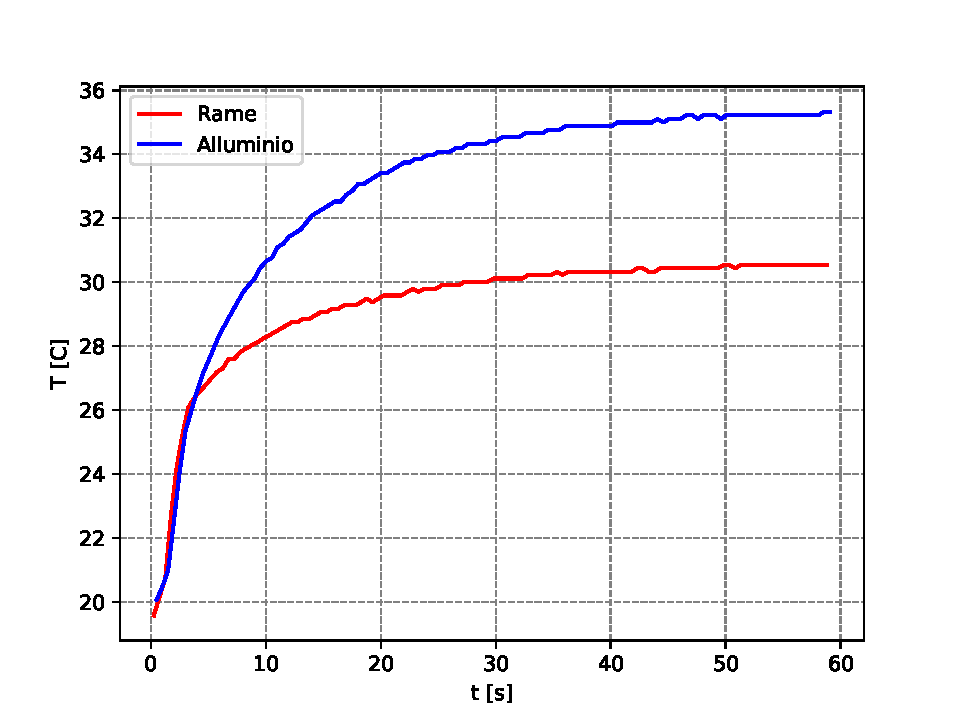
\includegraphics[width=0.8\textwidth]{extra/prima_misura.pdf}
        \caption{Grafico delle temperature misurate dalle termoresistenze in funzione del tempo.}
        \label{fig:prima_misura}
    \end{figure}
    Si nota subito che la temperatura segue una legge di potenza, come ci si può aspettare
    dalla teoria. Abbiamo manualmente interrotto la registrazione delle misure quando la
    temperatura delle termoresistenze si è stabilizzata, e abbiamo ripetuto l'operazione
    per ciascun foro.
    Infine abbiamo preso nota del diametro $d$ delle barre che risulta valere 
    , del voltaggio $V$ e della corrente $I$ passante per le resistenze,
    i valori ottenuti sono:
    \begin{itemize}
        \item $d=\SI{2.50(1)}{\cm}$
        \item $V=\SI{1.0(1)}{\volt}$
        \item $I=\SI{1.0(1)}{\ampere}$
    \end{itemize}
    \section{Elaborazione dei dati}
    I dati ricavati sono riportati nel grafico in figura \ref{fig:temperature}, in cui le temperature sono
    mostrate in funzione della distanza dalla fonte fredda.\\
    \begin{figure}[t]
        \centering
        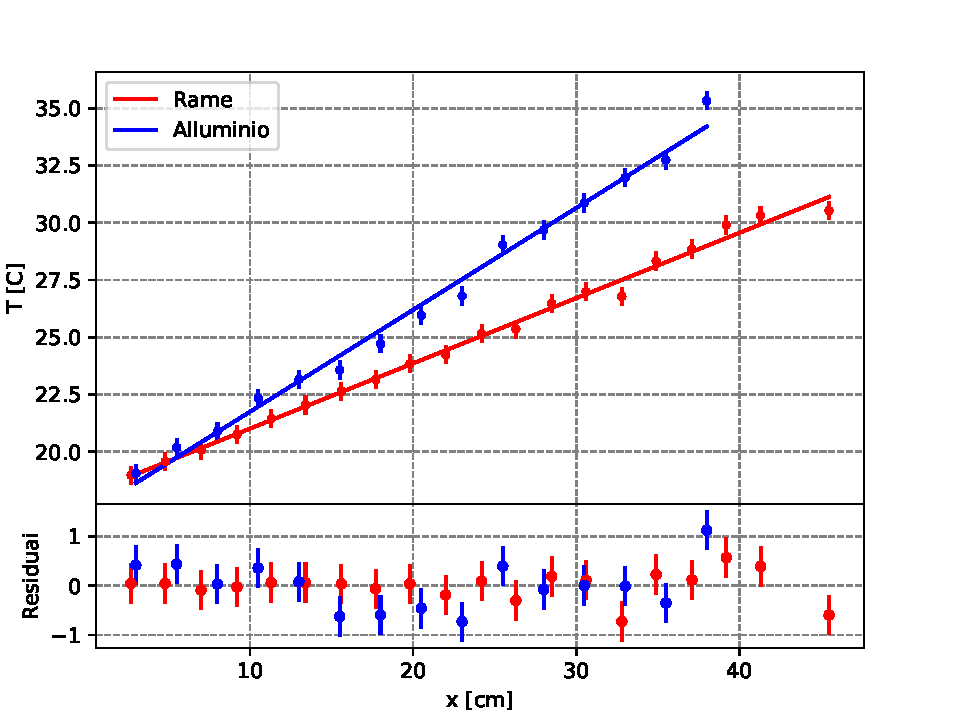
\includegraphics[width=0.8\textwidth]{extra/temperature.pdf}
        \caption{Grafico delle temperature dei due cilindri metallici in funzione della
        distanza dalla fonte fredda}
        \label{fig:temperature}
    \end{figure}
    La teoria prevede che la temperature $T_i$, misurata ad una distanza $x_i$ dalla
    fonte fredda vale:
    \begin{equation}
        \label{eq:T_i}
        T_i=T_0+\frac{W}{ \lambda S}x_i
    \end{equation}
    dove $T_0$ è la temperatura della fonte fredda, 
    $lambda$ è la conducibilità termica del materiale,
    $S$ è l'area della sezione della barra e 
    $W$ è il flusso di calore, ovvero la quantità di calore trasmesso dalla barra per 
    unità di tempo.\\
    Per prima cosa possiamo ricavare il valore di $W$; supponendo che lo scambio di calore
    con l'ambiente sia trascurabile, $W$ è pari alla potenza dissipata dalla resistenza,
    che si può esprimere in funzione della tensione $V$ e della corrente $I$,
    dato che il nostro apparato consisteva in due resistenze in parallelo si ha:
    \begin{equation}
        W=\frac{VI}{2}\approx\SI{0.5(1)}{\watt}
    \end{equation}
    Abbiamo quindi fittato i dati sperimentali alla \ref{eq:T_i} attraverso un programma
    in python che fa uso della funzione 
    \href{https://docs.scipy.org/doc/scipy/reference/generated/scipy.optimize.curve_fit.html}{curve\_fit}
    della libreria scipy. 
    Il coefficiente angolare $k$ restituito dalla funzione risulta quindi essere una
    stima della quantità $\frac{W}{ \lambda S}$, da cui possiamo ricavare il valore
    della conducibilità termica $\lambda$:
     \begin{equation}
        \lambda= \frac{W}{kS}\approx
    \end{equation}

    \section{Conclusioni}

\end{document}
